\documentclass[conference]{IEEEtran}
\IEEEoverridecommandlockouts
\usepackage{cite}
\usepackage{amsmath,amssymb,amsfonts}
\usepackage{algorithmic}
\usepackage{graphicx}
\usepackage{textcomp}
\usepackage{xcolor}
% \usepackage{natbib}

\begin{document}

  \makeatletter
  \newcommand{\linebreakand}{
    \end{@IEEEauthorhalign}
    \hfill\mbox{}\par
    \mbox{}\hfill\begin{@IEEEauthorhalign}
  }
  \makeatother

  \title{Sistema control modelo}

  \author{
    \IEEEauthorblockN{
        1\textsuperscript{st}  Martinez, Brayan Steven
    }
    \IEEEauthorblockA{
        \textit{Ingeniería Mecatrónica} \\
        \textit{Universidad EIA}\\
        Medellín, Colombia \\
        brayan.martinez@eia.edu.co
    }
    \and
    \IEEEauthorblockN{
        2\textsuperscript{nd} Gongora, Juan Pablo
    }
    \IEEEauthorblockA{
        \textit{Ingeniería Mecatrónica} \\
        \textit{Universidad EIA}\\
        Medellín, Colombia \\
        juan.gongora@eia.edu.co
    }
    \and
    \IEEEauthorblockN{
        3\textsuperscript{rd} aaa, aaaa aaaa
    }
    \IEEEauthorblockA{
        \textit{Ingeniería Mecatrónica} \\
        \textit{Universidad EIA}\\
        Medellín, Colombia \\
        email
    }
    \and
    \IEEEauthorblockN{
        4\textsuperscript{th} aaa, aaaa aaaa
    }
    \IEEEauthorblockA{
        \textit{Ingeniería Mecatrónica} \\
        \textit{Universidad EIA}\\
        Medellín, Colombia \\
        email
    }
    \and
    \IEEEauthorblockN{
        5\textsuperscript{th} aaa, aaaa aaaa
    }
    \IEEEauthorblockA{
        \textit{Ingeniería Mecatrónica} \\
        \textit{Universidad EIA}\\
        Medellín, Colombia \\
        email
    }
    \and
    \IEEEauthorblockN{
        6\textsuperscript{th} aaa, aaaa aaaa
    }
    \IEEEauthorblockA{
        \textit{Ingeniería Mecatrónica} \\
        \textit{Universidad EIA}\\
        Medellín, Colombia \\
        email
    }
  }
  \maketitle

  \begin{abstract}
    Ut id augue ut ex convallis blandit quis ac libero. Donec ante nunc, dictum non erat id, pharetra tempus nunc. Cras eget dignissim sapien. Vestibulum convallis dolor non odio vestibulum sagittis. In hac habitasse platea dictumst. Praesent varius arcu quis quam hendrerit, a euismod elit gravida. Ut dapibus vulputate elementum. Aliquam posuere et nibh ut molestie.
  \end{abstract}

  \begin{IEEEkeywords}
    \LaTeX, robotica, otra
  \end{IEEEkeywords}

  \section{Introducción}
  Lorem ipsum dolor sit amet, consectetur adipiscing elit. Aenean et tortor ornare, mattis augue vitae, vestibulum nulla. Ut lacus orci, viverra nec lectus consequat, laoreet luctus neque. Donec scelerisque ante ac fringilla malesuada. Cras porttitor lectus erat, at convallis ex cursus a. Ut vehicula eget magna sit amet mattis. Cras at fermentum mauris, semper luctus nibh. Nunc consectetur scelerisque tellus at volutpat. Nullam ut vulputate urna. Donec sem elit, blandit quis cursus ut, ullamcorper nec sapien. Sed mauris elit, mattis sed luctus ut, tristique ac libero. Donec a sollicitudin urna, at congue nulla. Nulla a blandit dolor, ut vehicula sapien. Donec at augue diam. Quisque turpis eros, luctus id aliquam efficitur, pulvinar sit amet magna. Fusce at dui tortor.
  
  \section{Materiales y método}
  Programas como Matlab para realizar matemática computacional y CoppeliaSim para realizar simulación física de robots
  Modelo Cinemático \cite{tejada}
  
  \section{Resultados}
  \subsection{Simulación Matlab}
  Se obtiene una primera simulación numérica usando Matlab.
  El robot comienza en (0,0) a 90° de la horizontal, se desea que llegue a (1.5, 3.2).
  El resultado se puede ver en la Figura \ref{fig:robotpos}. La orientación del robot
  se va alineando con el vector definido por el punto inicial y final.

  \begin{figure}
    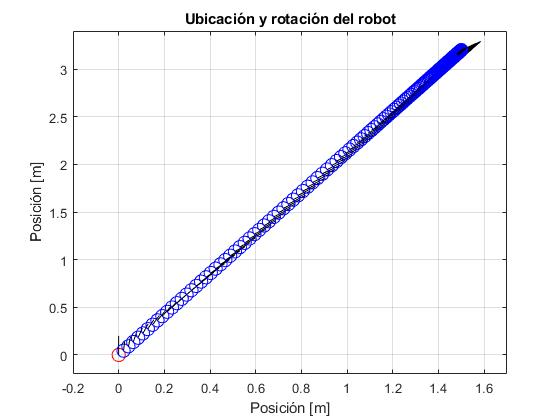
\includegraphics[width=\linewidth]{figures/matlab_pos_1.jpg}
    \caption{Registro de movimiento del robot}
    \label{fig:robotpos}
  \end{figure}


  Aprovechando el modelo cinemático, se puede graficar la velocidad angular de
  los motores, como se observa en la Figura \ref{fig:motorang}, la velocidad se reduce hasta 0,
  llegando así a la posición final.
  
  \begin{figure}
    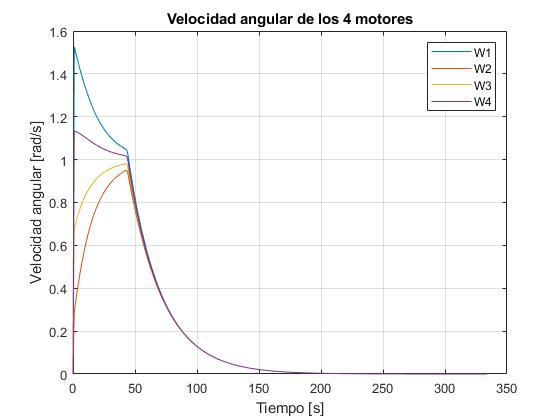
\includegraphics[width=\linewidth]{figures/matlab_motor_1.jpg}
    \caption{Velocidad angular de los motores en el tiempo}
    \label{fig:motorang}
  \end{figure}
  
  \subsection{Simulación CoppeliaSim}
  Se obtiene también, una simulación virtual en base al modelo cinemático y un robot con el cual se prueba el modelo.
  En CoppeliaSim se dispone del KUKA YouBot que viene por defecto, una plataforma con ruedas omnidireccionales.
  
  \begin{figure}
    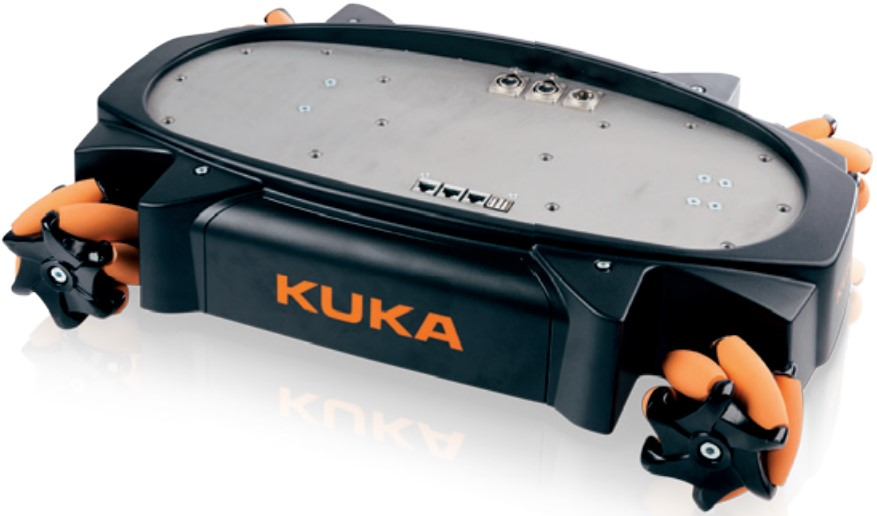
\includegraphics[width=\linewidth]{figures/kuka_real_youbot.jpg}
    \caption{KUKA YouBot en la realidad}
    \label{fig:kukayoubot}
  \end{figure}

  \begin{figure}
    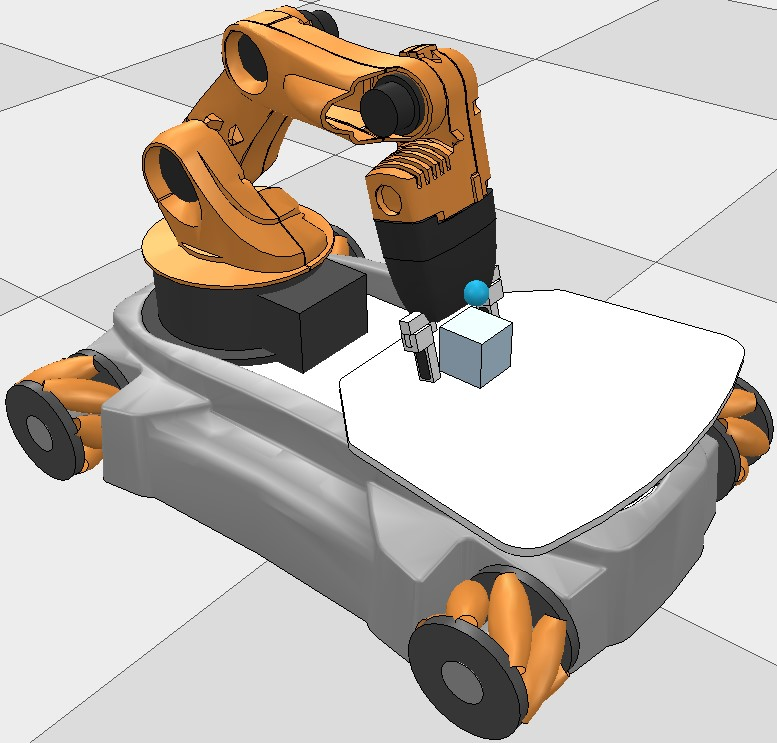
\includegraphics[width=\linewidth]{figures/kuka_sim_youbot.jpg}
    \caption{KUKA YouBot en CoppeliaSm}
    \label{fig:kukayoubot}
  \end{figure}
  
  \begin{figure}
    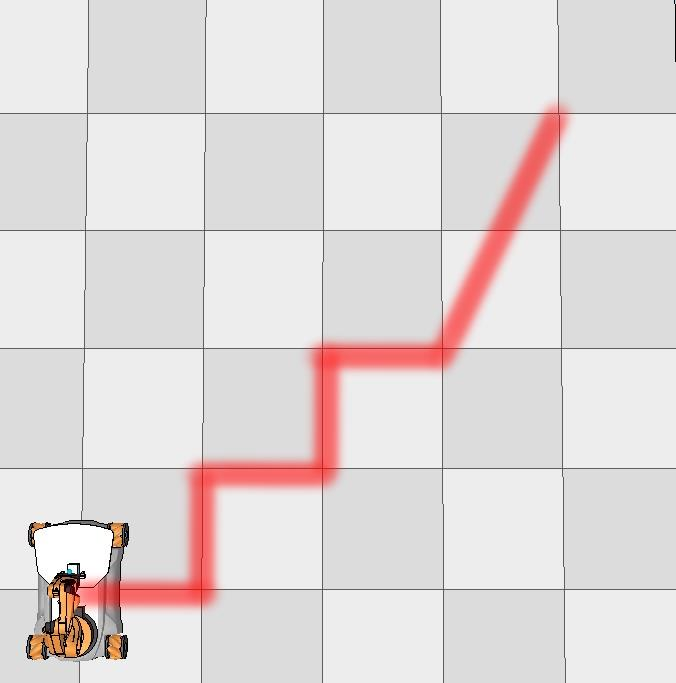
\includegraphics[width=\linewidth]{figures/kuka_init_pos.jpg}
    \caption{Ruta programada para el KUKA YouBot y posición inicial}
    \label{fig:kukaroute}
  \end{figure}

  \begin{figure}
    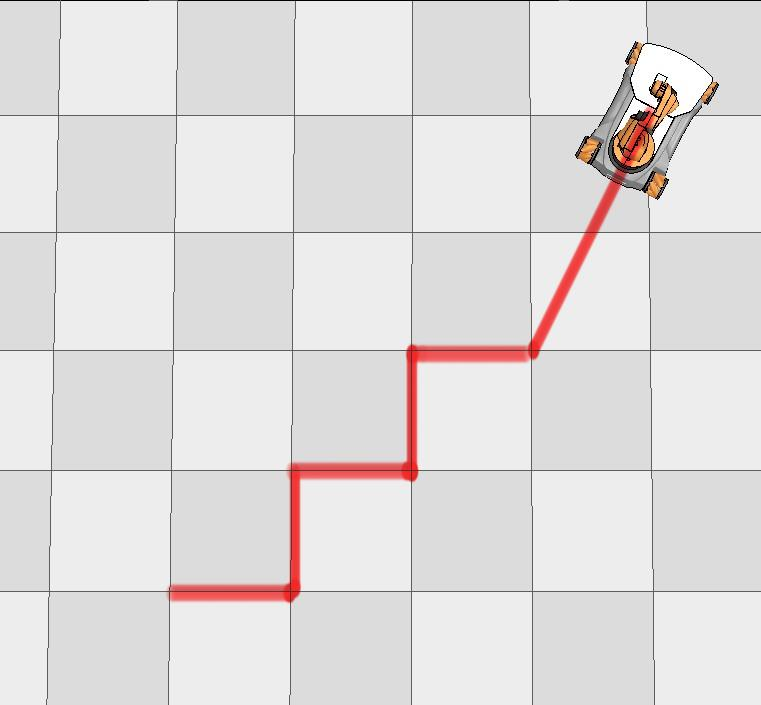
\includegraphics[width=\linewidth]{figures/kuka_final_pos.jpg}
    \caption{Posición final KUKA YouBot}
    \label{fig:kukafinal}
  \end{figure}

  Se programó un desplazamiento como en la Figura \ref{fig:kukaroute} donde al final
  se incluye una rotación y se puede visualizar en la Figura \ref{fig:kukafinal}

  \subsection{Aprendizajes en ROS}
  \subsection{Revisión Odroid}
  \section{Discusión o análisis de resultados}
  Lorem ipsum dolor sit amet, consectetur adipiscing elit. Aenean et tortor ornare, mattis augue vitae, vestibulum nulla. Ut lacus orci, viverra nec lectus consequat, laoreet luctus neque. Donec scelerisque ante ac fringilla malesuada. Cras porttitor lectus erat, at convallis ex cursus a. Ut vehicula eget magna sit amet mattis. Cras at fermentum mauris, semper luctus nibh. Nunc consectetur scelerisque tellus at volutpat. Nullam ut vulputate urna. Donec sem elit, blandit quis cursus ut, ullamcorper nec sapien. Sed mauris elit, mattis sed luctus ut, tristique ac libero. Donec a sollicitudin urna, at congue nulla. Nulla a blandit dolor, ut vehicula sapien. Donec at augue diam. Quisque turpis eros, luctus id aliquam efficitur, pulvinar sit amet magna. Fusce at dui tortor.
  
  \section{Conclusión}
  Lorem ipsum dolor sit amet, consectetur adipiscing elit. Aenean et tortor ornare, mattis augue vitae, vestibulum nulla. Ut lacus orci, viverra nec lectus consequat, laoreet luctus neque. Donec scelerisque ante ac fringilla malesuada. Cras porttitor lectus erat, at convallis ex cursus a. Ut vehicula eget magna sit amet mattis. Cras at fermentum mauris, semper luctus nibh. Nunc consectetur scelerisque tellus at volutpat. Nullam ut vulputate urna. Donec sem elit, blandit quis cursus ut, ullamcorper nec sapien. Sed mauris elit, mattis sed luctus ut, tristique ac libero. Donec a sollicitudin urna, at congue nulla. Nulla a blandit dolor, ut vehicula sapien. Donec at augue diam. Quisque turpis eros, luctus id aliquam efficitur, pulvinar sit amet magna. Fusce at dui tortor.
  
  Pellentesque placerat nunc at sapien accumsan scelerisque. Donec a dignissim justo, a aliquam metus. Donec mattis bibendum magna, et euismod justo pretium ut. Ut sed ultricies massa, in finibus arcu. Aliquam erat volutpat. Nunc elementum vehicula justo, non placerat elit. Nulla in felis dui. Ut sollicitudin ornare diam, ut blandit sapien interdum ac. Nam suscipit felis vitae ligula ornare volutpat. Suspendisse cursus ornare placerat. Morbi mollis nulla leo, et vehicula nulla iaculis ac. Nulla nec est porta, facilisis lectus nec, vulputate turpis. Quisque sollicitudin, nunc non sodales tincidunt, erat neque luctus eros, ac eleifend leo massa id felis. Nullam feugiat ornare leo in consequat. Curabitur ultrices luctus felis, id tempor augue venenatis at. Donec sed augue justo.
  
  \newpage

  \bibliography{references}
  \bibliographystyle{IEEEtran}

\end{document}